\documentclass[a4paper,11pt]{article}


% % % % % % % % % % % % % % % % % % % % % % % % % % % % %
% % ATTENTION : dans les figures le label doit être mis 
%APRES le caption pour que le numéro de la figure lorqu'on
%la référence soit le bon ; sinon on a le numéro du paragraphe
% % % % % % % % % % % % % % % % % % % % % % % % % % % % %

% package qui fournit \justify 
\usepackage[document]{ragged2e}

%pifont pour les puces de formes spéciales
\usepackage{pifont}

% césure exemple
% \hyphenation{an-ti-cons-ti-tu-tion-nel

\usepackage[utf8x]{inputenc}
\usepackage[T1]{fontenc}
\usepackage[frenchb]{babel} % If you write in French
%\usepackage[english]{babel} % If you write in English
\usepackage{lmodern} % Pour changer le pack de police
\renewcommand*\familydefault{\sfdefault}
\usepackage{makeidx}
\usepackage{amsthm}
\usepackage{amsmath}
\usepackage{amssymb}
\usepackage{mathrsfs}
\usepackage{stmaryrd}
\usepackage{geometry}
%\usepackage{graphicx}
\usepackage{graphbox}
\usepackage{supertabular}
\usepackage{tabularx}
\usepackage{longtable}
\usepackage{pdflscape}
\geometry{hmargin=2cm,vmargin=2cm}

\usepackage{booktabs}
\usepackage{tabularx}
\usepackage[table]{xcolor}
\usepackage{ltablex}
\usepackage{float}
\usepackage{url}

\usepackage{chngcntr}
\counterwithin*{footnote}{page}


\usepackage[titletoc,toc,title,page]{appendix}
\renewcommand{\appendixtocname}{Annexes}
\renewcommand{\appendixpagename}{Annexes}

\usepackage{standalone}
\usepackage{ifthen}
\usepackage{xstring}
\usepackage{calc}
\usepackage{pgfopts}
\usepackage{tikz}
\usetikzlibrary{positioning,shapes,shadows,arrows}

\usepackage{algpseudocode}
\usepackage{algorithm}
\makeatletter
\renewcommand{\ALG@name}{Algorithme}
\renewcommand{\listalgorithmname}{Table des algorithmes}

\newtheorem{theo}{Définition}[section]
\usepackage{mathtools, bm}
\usepackage{amssymb, bm}

\usepackage{hyperref}
\hypersetup{
    colorlinks=true,       % false: boxed links; true: colored links
    linkcolor=black,       % color of internal links
    citecolor=purple,       % color of links to bibliography
    urlcolor=blue          % color of external links
}

\usepackage{listings}

\definecolor{dkgreen}{rgb}{0,.6,0}
\definecolor{dkblue}{rgb}{0,0,.6}
\definecolor{dkyellow}{cmyk}{0,0,.8,.3}

\lstset{
  language        = php,
  basicstyle      = \small\ttfamily,
  keywordstyle    = \color{dkblue},
  stringstyle     = \color{red},
  identifierstyle = \color{dkgreen},
  commentstyle    = \color{gray},
  emph            =[1]{php},
  emphstyle       =[1]\color{black},
  emph            =[2]{if,and,or,else},
  emphstyle       =[2]\color{dkyellow}}



\usepackage{blindtext}
\usepackage{enumitem} % pour changer les puces dans \itemize


\date{\today}

\makeindex
\def\siecle#1{\textsc{\romannumeral #1}\textsuperscript{e}}
\newcommand{\argmax}{\mathop{\mathrm{argmax}}\nolimits}
\newcommand{\pgcd}{\mathop{\mathrm{pgcd}}\nolimits}

\makeatletter
\renewcommand{\pod}[1]{\allowbreak\mathchoice
  {\if@display \mkern 18mu\else \mkern 8mu\fi (#1)}
  {\if@display \mkern 18mu\else \mkern 8mu\fi (#1)}
  {\mkern4mu(#1)}
  {\mkern4mu(#1)}
}

\usepackage{wallpaper}

\begin{document}
\renewcommand{\labelitemi}{\textbullet}
% pour factoriser l'échelle des figures 
%utilisation scale=\scaledvwa au lieu de scale = 0.3 ... 
\newcommand{\scaledvwa}{0.4} 
\newcommand{\scaledvw}{0.3}
\newcommand{\scalekad}{0.45}


\phantomsection
\begin{titlepage}
	\parindent=0pt
\ThisTileWallPaper{1.3\paperwidth}{1.0\paperheight}{images/fret}
 
\addtolength{\wpXoffset}{-4.5cm}

%	\vspace*{\stretch{1}}
%	\begin{center}
%		
\includegraphics[scale=0.5]{images/enac.png}%
%	\end{center}
	
\color{white}{	\vspace*{\stretch{1}} }
	\hrulefill
	\begin{center}\bfseries\Huge
		\color{white}
		{Analyse stratégique des Sociétés de Fret Aérien Civil Traditionnelles} 
	\end{center}
	\hrulefill
	
	\vspace*{1cm}
	\begin{center}\bfseries\Large
			\color{white}
		{Florian Barbarin - Abdelkader Beldjilali - Nicolas Holvoet}
		
	\end{center}
	
	\vspace*{\stretch{2}}


\end{titlepage}%on créé la couverture

\pagebreak

\tableofcontents
\justify

\pagebreak

\section*{Introduction}
\addcontentsline{toc}{section}{Introduction}

Le transport aérien de fret s'est développé à partir de 1911 lors d'un
premier vol dont l'objet était de livrer 15 kg de courrier entre deux villes asiatiques distantes de 10 km sur un biplan Sommer. 

%Depuis, le traffic a "légèrement" augmenté pour atteindre en 2014, 51 millions de tonnes pour une valeur de US\$6.8 trillions \cite{RePEc:eee:jaitra:v:61:y:2017:i:c:p:34-40}.

Aujourd'hui, le fret aérien, au même titre que le transport de passagers, continue de jouer un rôle majeur dans l'économie, le développement international et plus fondamentalement dans notre manière d'appréhender le monde au même titre que son pendant virtuel, l'Internet. 


%La présente étude vise à effectuer une analyse de marché suivant le modèle des 5 forces de Porter.
%Le modèle de Porter consiste à effectuer l'analyse de marché suivant 5 domaines :
%la concurrence dans le secteur, deux menaces : les nouveaux entrants et les substituts et deux déterminants : pouvoir de marché des clients et fournisseurs.
%
%\begin{figure}[H]
%	\begin{center}
%		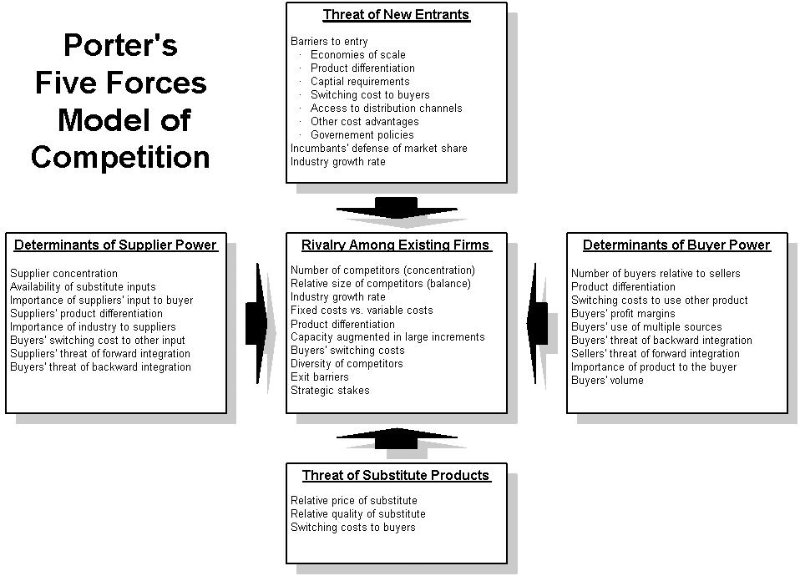
\includegraphics[scale=0.48]{images/porter/porter_1}
%		\caption{Modèle de Porter}
%		\label{inclusion}
%	\end{center}
%\end{figure}
%
%
%Suivront une étude du rôle de l'Air Traffic Management (ATM) dans la stratégie des acteurs du secteur et de son évolution future au regard de ces stratégies des acteurs du secteur. 
%   





\section{Analyse de marché suivant le modèle de Porter}

\subsection{Concurrence entre les firmes existantes}

\subsubsection{Définition du marché}

Le marché concerne le fret aérien qui désignera dans la suite tous les biens y compris le fret postal à l’exception des bagages. (IATA)

Cette étude porte sur les sociétés de Fret Aérien Civil Traditionnelles (FACT) qui gèrent leur propre flotte aérienne pour le transport de biens. Ce qui exclut le fret militaire ainsi que les logisticiens, entreprises de fret "virtuelles", qui font souvent du point à point par le biais de location de charters ou d'achat d'emplacements aux compagnies de fret traditionnelles. Les compagnies virtuelles constituent donc à la fois des clients pour les acteurs de Fret Aérien Civil Traditionnel (FACT) en leur permettant d'optimiser le remplissage de leurs avions-cargo, mais aussi une forme de concurrence puisque le fret transporté au nom du logisticien est "perdu" pour tous les transporteurs classiques, y compris celui qui assure réellement le service.



\subsubsection{Description des produits concernés}
\label{produits}
Pour évaluer la concurrence, il convient d'étudier en premier lieu le type de produits transportés. En effet, le pétrole ou le gaz, ne sont pas en général, transportés par avions ; sur ces matières premières, le fret aérien ne concurrence pas les secteurs maritimes, routiers, ferroviaires, fluviaux ou par oléoduc/gazoduc. 

Le fret aérien, pour être compétitif, concerne donc les produits à haut rapport valeur-poids, souvent aussi à forte valeur ajoutée, ou à forte contrainte temporelle :


\begin{itemize}
	\item Électronique,
	\item Produits périssables : fleurs, fruits...
	\item Produits urgents (colis express...) ou à finalités humanitaires.
\end{itemize}



\subsubsection{Taxonomie des acteurs du transport du fret}
\label{taxonomie}
On distingue 3 types de sociétés de transport qui exhibent des structures de coûts, des caractéristiques opérationnelles et une répartition spatiale de l'offre et de la demande distinctes.\\


Les \textbf{compagnies de cargo} qui ont pour cœur de métier le seul transport aérien de fret, principalement sur les liaisons long-courriers ou transatlantiques. Ces compagnies possèdent une flotte d'avions tout-cargo dédiés, qui vont du gros porteur B747-8F de rayon d'action 8000 km et de capacité 140 tonnes, au Beluga – Airbus A300 reconverti – jusqu'au simple twin turboprop Cessna super cargomaster (RA : 1700 km, capacité de fret : 1.8 tonnes). Un transporteur de fret classique comme Cargolux a très peu de frais de personnel et de frais commerciaux. En revanche, les coûts liés aux avions, aux redevances aéronautiques et aux frais d’escale sont élevés. Seuls 10 à 15 \% du trafic mondial de fret aérien est réalisé par ce type de compagnies. \cite{popescu}\\
	
Les \textbf{compagnies mixtes} telles que Lufthansa, Air France-KML ou encore Emirates et Korean Air utiliseront soit le transport en soute dans leurs avions-passagers, soit des avions cargo combinés, i.e. des avions configurés de manière permanente pour le transport de fret et de PAX ou des avions reconfigurables rapidement pour les deux types de transport. Pour illustrer le transport en soute, on note qu'un moyen-courrier assurant un vol avec 200 passagers représente un revenu d’environ US\$100 000, auxquels s’ajouteront quelque US\$13 000 en fonction du taux de remplissage des soutes de l’avion. Un moyen-courrier de la catégorie A330/B767 permet d’embarquer environ 10 tonnes de fret hors bagages. En 2015, la valeur moyenne de chaque kilo transporté par avion s’établit à US\$127, contre US\$1,10 pour le maritime.
Certaines compagnies mixtes possèdent aussi des filiales spécialisées dans le cargo. On peut citer par exemple Emirates SkyCargo, classée 3e en terme de fret tonne-kilomètres (FTK) ou British Airways World Cargo classée 12e. Mais même dans ce contexte, British Airways va cesser l'exploitation de ses Boeing 747-8F dédiés pour se recentrer sur les opportunités qu'offre le cargo en soute. \cite{theEconomist01}\\

Les \textbf{intégrateurs}\label{integrateurs} comme FedEx, UPS, TNT ou DHL, qui font du point à point avec des avions tout-cargo via des hubs dédiés, sont des entreprises avec des frais de personnel plus élevés et des coûts avion moindres grâce à une flotte d'appareils d’occasion convertis en cargo : A300-600, A310. \cite{lantenne} Dans leur logique du dernier kilomètre, ces intégrateurs opèrent une chaîne logistique multimodale complète en disposant également de leurs propres entrepôts, camions et maillages routiers.\\

On remarque que le transport de fret en soute peut être facturé au coût marginal car les coûts directs d'exploitation du vol sont imputés aux passagers, ce qui lui offre un avantage concurrentiel sur le tout-cargo. Trois solutions possibles à ce problème : la régulation des prix pour protéger les tout-cargo, le ré-ajustement de la flotte pour les compagnies mixtes qui revendent leur cargo, voire constituent des filiales disjointes, ou la différentiation en offrant des services spécifiques. Ce dernier point vaut notamment pour les entreprises tout-cargo qui ne sont pas astreintes à opérer sur des aéroports destinés au trafic passager ; il s'agit ici de tirer partie
de la souplesse dans la localisation et la topologie du réseau mondial de hubs de fret. Dans ce sens, nous verrons que les intégrateurs ont su s'imposer sur le marché en apportant une solution clé en main.


Enfin, les compagnies mixtes sont soumises à une barrière de sortie du secteur du fret beaucoup plus souple et rentable. Les tout-cargo, quant à elles, n'ont d'autres choix que le rachat par un concurrent ou nouvel entrant, de mettre la clé sous la porte, d'évoluer ou de fusionner. À l'instar du transport de passagers, des alliances permettent des économies d'échelles et des synergies bénéfiques en terme de qualité et versatilité des services proposés au clients. Des ententes illégales sur le prix du fret ont été révélées il y a quelques années, entre Qantas Airways et plusieurs autres compagnies ou encore Air France-KLM, Cathay Pacific et SAS Cargo...\cite{popescu}


\subsubsection{Description du marché}
Le fret aérien génère un chiffre d’affaires annuel évalué par l’Association internationale du transport aérien (IATA) à 47,8 milliards de dollars en 2016. Les avions ont embarqué 53,9 millions de tonnes de fret en 2016. L’aérien ne représente qu’un faible pourcentage du volume du fret (environ 5 \%),
mais environ 35 à 40 \% en valeur. \cite{lantenne}. Ce secteur demeure toutefois une activité minoritaire au sein des compagnies aériennes, le transport de passagers produisant 80 à 85 \% de ses recettes. Le transport maritime constitue le principal concurrent de l’aérien. Du fait de son coût très faible, les entreprises optimisent leur logistique pour rendre compatibles les délais de transport avec leur activité. Les autres modes de fret, a contrario, se présentent parfois comme complémentaires de l'aérien : fret camionné de Toulouse au hub de Roissy-CDG par exemple.

En terme de taille de marché, on comptait en 2015 environ 200 firmes spécialisées dans le cargo, y compris les intégrateurs définis § \ref{taxonomie}, auquel s'ajoute un nombre approximatif de 1100 compagnies aériennes dédiées au transport de passagers et appelées de plus en plus à alimenter l'offre en fret AFTK (Available Fret Tonne-Km) ; les \textit{wide-body} aux capacités en soute augmentée n'y sont pas étrangers.

En 2014, la part de marché en valeur, en revenu tonne kilomètre global (RTK), pour le tout-cargo (compagnies de cargo et intégrateurs) se monte à 56 \%. La tendance depuis 2000 est à la baisse au profit des compagnies mixtes avec transport en soute, avec probablement une part de marché en quantité qui ne dépasse pas désormais les 30 \%. L'adverbe \textit{probablement} souligne ici la difficulté d'obtention et d'interprétation des données aéronautiques. Le tout-cargo est en outre confronté au problème de la \textit{bi-directionnalité} c'est-à-dire au retour à vide après livraison, spécificité qui n'existe pas dans le transport de passagers, et que seules des optimisations en termes de flux et de placement des hubs permettent de soulager.

Pour donner une idée de la répartition des acteurs sur le marché, à défaut de pouvoir obtenir des données plus précises, on remarque en 2014 la prédominance des intégrateurs FedEx (7 millions de tonnes transportés) et UPS (4 Mt) et des compagnies asiatiques et du Moyen-Orient, hub des pays du Golfe : Emirates, Korean Air, Cathay Pacific Airways à Hong-Kong. \cite{top50}

L'évolution du marché est caractérisée par une croissance molle au niveau global et un contraste géographique marqué dû notamment aux hubs du Moyen-Orient et d'Asie. Sans développer davantage, on peut noter que la croissances du fret et du trafic passagers dans ces régions induit un accroissement du surplus de l'offre en fret (AFTK). Chaque mise en service d'un Boeing 777 ajoute 25 tonnes de fret 
à l'offre déjà surdimensionnée grevant ainsi la santé globale du secteur. \cite{theEconomist01}


Au niveau stratégique, le secteur est confronté à divers facteurs : sécurité, environnement, politiques protectionnistes, accords internationaux... L'accord de Bali (décembre 2013) visant à libéraliser les échanges commerciaux en réduisant la bureaucratie aux frontières et en aidant les pays les moins avancés pourrait par exemple multiplier le volume de fret aérien d'un facteur de 1.4 grâce à une baisse généralisée des coûts. \cite{iata.org01} On citera pour finir l'importance
de l'évolution de l'offre aéroportuaire pour éviter les problèmes de congestion.
Le climat peut en être une cause avec un nombre croissant d'aéroports inondables : 40 en Europe, 20 rien qu'en Norvège.
\subsection{Clients}

La nature des clients dépend fortement du type de modèle.

Les intégrateurs s'adressent directement aux entreprises ou aux individus, lesquels attachent une importance particulière à la logistique simplifiée porte-à-porte et aux délais de livraison garantis par une offre multimodale riche. Par ailleurs, les principaux intégrateurs ne se limitent pas au transport aérien et peuvent espérer tirer profit d'autres activités et toucher une clientèle élargie et fidélisée pour laquelle le transport aérien n'est plus une fin.

Les clients directs des compagnies de cargo ou des compagnies mixtes seront des logisticiens qui disposent des infrastructures et équipements nécessaires à la manutention du fret. Le surplus dans l'offre en capacité de fret conduit à une situation où le client
possède un fort pouvoir de négociation : non captif, le client peut changer facilement de fournisseur de service de fret aérien. Ainsi, les compagnies de fret n'ont parfois d'autre choix que de brader leurs prix.

En terme de taille de marché, les États-Unis en 2016 arrivent en tête avec 7.7 millions de tonnes de fret, suivis par l'Allemagne (4.4 Mt), la Chine (3.4 Mt) et Hong-Kong (3.2 Mt), de source IATA.


\subsection{Fournisseurs}

Comme pour toutes les compagnies aériennes, la volatilité et le niveau des prix du pétrole est un souci permanent, compensable cependant par des investissements financiers et les solutions alternatives, réacteur à gaz ou à biocarburant, qui ne sont encore qu'à l'état de prototypes. Les contraintes réglementaires et environnementales imposent également de renouveler les flottes avec des avions plus récents.

Au niveau des constructeurs d'avions, les entreprises de fret sont, peu ou prou, confrontées au duopole Boeing - Airbus. Elles possèdent malgré tout d'une part un pouvoir de négociation proportionnel à leur taille et d'autre part la possibilité de se fournir sur le marché de l'occasion ou de faire appel à la location.

Le secteur du fret est un consommateur captif vis-à-vis des fournisseurs de services aéroportuaires. Les contraintes de volume et de poids imposent des équipements spécifiques permettant de garantir une manutention sûre et efficace, aussi bien pour les phases de (dé)chargement que par l'utilisation d'enceintes à rayons X adaptées. Les sociétés de fret sont aussi dépendantes des créneaux qui lui sont attribués et doivent faire face à la congestion du trafic en travaillant avec les différents acteurs aéroportuaires et de l'ATM. Ceux-ci peuvent alors être perçus comme des compléments auxquels il est difficile de s'abstraire totalement, bien qu'il soit possible dans un premier temps d'opérer tout ou partie d'une plate-forme aéroportuaire dédiée au fret.

Enfin, les compagnies de cargo doivent, pour rester attractives face aux compagnies mixtes et aux intégrateurs, contracter des accords avec des logisticiens pour proposer des services annexes tels que le transfert routier.
\subsection{Menaces d'éventuels entrants}

Pour les intégrateurs, les barrières à l'entrée semblent davantage relever de la présence de mastodontes tels que FedEx, UPS, TNT ou DHL capables de pratiquer des prix bas dûs aux économies d'échelles et disposant d'une forte intégration internationale et locale avec des hubs et maillages routiers optimisés. 


En outre, si la possibilité de louer ses avions plutôt que de les acheter permet de créer des compagnies ariennes fussent-elles éphémères, la sur-capacité actuelle de l'offre favorise plutôt la sortie que l'entrée. Si la demande est destinée à augmenter, la capacité l'est également avec le nombre croissant de \textit{wide-body} en circulation. Les compagnies souhaitant expérimenter le modèle mixte devront ainsi justifier d'un solide réseau de routes et de hubs, ce qui explique aujourd'hui la prépondérance des majors dans ce marché.  

A priori, les nouveaux entrants éventuels se porteront plutôt sur des marchés de niche, à moins qu'ils ne surfent sur l'apport de nouvelles technologies telles que les drones, les avions sans pilotes, le tout numérique pour réduire le coût des formalités et les accélérer, le centraliser. Mais alors les firmes en place ne sont-elles pas les mieux placées pour tirer partie de ces avancées quitte à racheter ces start-up ?
\subsection{Menaces liées à l'existence de substituts}
\label{substituts}

Par son coût élevé, le transport de fret aérien se justifie dans le cadre de certains produits typiques définis au § \ref{produits} pour lesquels il n'existe généralement pas de substituts satisfaisants.

Cependant, dans certains cas, l'optimisation et l'anticipation logistique des entreprises peuvent leur permettre d'être moins dépendantes du transport aérien. Avec des progrès techniques, en termes de conservation et de chaîne du froid par exemple, le transport maritime peut aussi parfois devenir une option viable. Le transport ferroviaire, que l'on estime 80 \% moins cher que le transport aérien, continue lui aussi de se développer notamment entre l'Europe et l'Asie, concurrençant sérieusement le transport maritime et grignotant peut-être demain le marché du fret aérien. \cite{lemonde_train}

Enfin, l'augmentation des coûts de production à l'étranger, le développement du protectionnisme avec les crises, les problématiques liées au respect de la propriété intellectuelle peuvent constituer autant de raisons pour les entreprise de relocaliser leur production. En ce sens, le transport terrestre redevient un concurrent sérieux. 

\section{Rôle de l'ATM dans la stratégie des acteurs du fret aérien}

%Single European Sky ATM Research (SESAR)

Du fait des spécificités propres au secteur du fret aérien, l'ATM joue un rôle important dans l'organisation et la stratégie des différents acteurs. En effet, nous allons voir que le fait de transporter des marchandises implique des problématiques parfois bien différentes de celles du transport de passagers.

\subsection{Un trafic réparti}

\subsubsection{Des vols ayant principalement lieu la nuit}

Comme le montre différents articles tels que \cite{popescu}, le fret aérien a, dès ses origines, été principalement organisé avec des vols ayant lieu la nuit. En effet, cela a plusieurs avantages du point de vue de l'organisation du trafic aérien. 

Tout d'abord, cette activité étant en grande partie organisée autour de grands hubs \cite{Walcott201764}, cela permet aux marchandises de transiter le jour vers ces centres névralgiques pour ensuite être redistribuées dans le monde entier dans des avions chargés en toute fin de journée. 

Ensuite, les marchandises n'étant pas soumises aux mêmes contraintes temporelles que les passagers, leur transport dans des vols de nuit permet de répartir le trafic tout au long d'une journée : les heures de pointe sont alors consacrées aux vols passagers et les créneaux disponibles la nuit aux vols cargo. Cela permet donc de ne pas rajouter de trafic lors de périodes de congestion puisque les marchandises peuvent, dans la plupart des cas, partir en plein milieu de la nuit.

Une organisation de nuit peut également permettre à des entreprises de transport de fret de réduire certains coûts et d'assouplir leur organisation. En effet, ces vols ayant lieu hors période de congestion, les redevances aéroportuaires et de contrôle aérien peuvent être moins élevées qu'en plein pic de trafic. De même, la demande étant moindre, l'allocation de créneaux s'en trouve grandement facilitée.

Enfin, cette organisation autour de vols de nuit permet à certains acteurs de diversifier leur activité. On peut citer en France l'exemple de ASL Airlines France (anciennement Europe Airpost) qui possède plusieurs B737-300 \textit{Quick-Change} lui permettant d'effectuer des vols passagers le jour et des vols de fret la nuit.\\

On voit donc que les différents acteurs du transport aérien de fret prennent en considération un certain nombre de problématiques liées à l'organisation générale du trafic aérien et décident alors d'organiser principalement leur activité la nuit. Nous allons cependant voir que d'autres problématiques ATM peuvent porter atteinte à ce mode de fonctionnement.

\subsubsection{Un trafic de nuit remis en cause}

Comme nous venons de le voir, les transporteurs aériens de fret utilisent essentiellement des créneaux de nuit pour leurs vols. Cependant, principalement pour des raisons de gêne des riverains, le trafic de nuit est remis en cause sur de nombreux aéroports. Par exemple, un couvre-feu est mis en place sur l'aéroport de Paris-Orly entre 23H30 et 6H00 depuis 1963 afin d'éviter le survol par les aéronefs des zones habitées en plein milieu de la nuit.

Il est à noter que sur certains aéroports, le trafic de nuit peut être malgré tout important du fait de la présence du hub de certaines compagnies de fret. C'est le cas notamment à Paris-Charles-de-Gaulle où FedEx et d'autres compagnies de fret ont leur hub. 

Les articles \cite{boutelet_2012} et \cite{garric_2012} montrent par exemple en quoi la fin des vols de nuit imposée à l'aéroport de Francfort peut porter atteinte au développement du trafic de fret aérien.

Dans ce cadre, les compagnies sont dans l'obligation de revoir leur stratégie vis-à-vis de l'organisation du trafic. Les départs des vols de fret doivent alors se faire plus tôt ou plus tard et, parfois, prendre part à la congestion à certaines périodes.

Cette réduction des possibilités de vols de nuit peut également pousser les compagnies vers une réduction de l'utilisation d'avions tout-cargo au profit de l'embarquement de fret sur les vols passagers. C'est en effet une tendence forte du secteur comme le montre \cite{RePEc:eee:jaitra:v:61:y:2017:i:c:p:34-40}. Même si cette tendance ne trouve pas forcément son origine dans la réduction des vols de nuit, cette nouvelle contrainte ne fait que favoriser ce changement de stratégie. Cela permet en effet d'optimiser l'utilisation des capacités de transport des aéronefs passagers en embarquant du fret qui aurait pu être transporté par un avion tout-cargo et donc de réduire le trafic des aéronefs entièrement dédiés au fret. L'article montre même que certaines compagnies, comme Air France, éliminent les avions tout-cargo de leur flotte au profit de ce mode de transport des marchandises.

Dans le cas où les aéroports continuent de permettre les vols de nuit, les problèmes de voisinage liés à ces vols ont d'autres impacts sur la gestion du trafic. Par exemple, de nombreux aéroports ont mis en place des procédures particulières pour que la gêne des riverains soit diminuée la nuit. Il s'agit dans la plupart des cas de nouvelles procédures aux instruments plus précises, évitant le survol de certaines zone voire obligeant les aéronefs à survoler un endroit précis au-dessus d'une certaine altitude. Ces procédures mises en place montrent bien le rôle que peut avoir l'ATM pour permettre aux compagnies de fret de continuer à voler la nuit sur certains aéroports.\\

On voit donc que des contraintes liées à la gestion du trafic de nuit peuvent imposer aux compagnies de fret de se réorganiser et de redéfinir en quelque sorte leur stratégie.

\subsection{Un réseau fortement maillé}

Comme le montre \cite{O'Kelly20141}, des compagnies de transport de fret comme FedEx bénéficient de plusieurs hubs dans le monde entier et d'un réseau de lignes très dense. Cela permet donc une optimisation très fine  du trafic et des coûts au sein de chaque compagnie. Voyons les implications que cela peut avoir du point de vue de l'ATM.

\subsubsection{Un "routage" facilité des marchandises}

La densité du réseau auquel ont accès les compagnies de fret permet du multiplier les chemins permettant, à partir d'un point A, d'arriver à un point B. En effet, une marchandise de FedEx partant de France et dont la destination finale est le centre des États-Unis pourra emprunter sans grande différence en terme de distance le hub de Memphis, d'Oakland ou d'Indianapolis.

Cela permet aux compagnies d'optimiser les différents chargements de leurs avions et, par là, de répartir sur différentes lignes les marchandises transportées, mais aussi de limiter le phénomène de retour à vide. Encore une fois, cela peut avoir des implications non négligeables en terme de gestion du trafic puisqu'au lieu de faire partir plusieurs avions vers une même destination, certaines charges transportées peuvent être réparties sur d'autres lignes déjà existantes.

Cette optimisation du "routage" des marchandises est, de plus, renforcée par le point qui suit.

\subsubsection{Un trafic très résilient face aux retards}

Comme nous avons déjà pu le remarquer, le transport de marchandises a pour spécificité de ne pas avoir les mêmes contraintes temporelles que les passagers.

En effet, lorsqu'un avion transportant des passagers est en retard ou annulé, un grand nombre de mesures doivent être mises en place pour la prise en charge de ces derniers et leur acheminement dans les meilleurs délais.

En ce qui concerne la plupart des marchandises, un retard de quelques heures n'a que très peu d'implications (sauf marchandises bien spécifiques comme dans le cas du transport d'animaux vivants). Ainsi, il est possible de faire le choix de routes rallongeant quelque peu le transport d'une marchandise sans que cela ait un réel impact sur le service rendu. Cela permet encore une fois d'optimiser la répartition des marchandises sur différentes lignes.

De même, les compagnies de fret étant, dans certains cas, très résilientes face aux retards, il leur est possible d'accepter, par exemple, des changements de créneau afin de désengorger le trafic sur un aéroport congestionné.\\

On voit donc en quoi la spécificité du transport aérien de fret a des implications sur la gestion générale du trafic aérien. Nous pouvons d'ailleurs également voir qu'un certain nombre de nouveaux développements dans l'ATM peuvent encore modifier les stratégies des acteurs du fret aérien.

\section{Rôle de l'ATM dans le futur par rapport aux stratégies des acteurs }

L'\textit{Air Traffic Management} est un domaine en perpétuelle évolution, tout particulièrement ces dernières années en Europe. En effet, il s'agit d'un secteur où les procédures et les outils doivent évoluer et s'adapter au trafic afin d'assurer une meilleure gestion du trafic tout en gardant un niveau de sécurité élevé. Nous allons voir un certain nombre d'évolutions qui pourraient avoir un impact sur les acteurs du fret aérien.

\subsection{L'opportunité du programme SESAR}

Comme le montre \cite{52008DC0750}, le programme \textit{Single European Sky ATM Research} (SESAR) mis en place par la Commission Européenne affiche d'ambitieux objectifs tels que :
\begin{itemize}
\item une réduction de moitié des coûts de contrôle aérien;
\item une réduction de 10\% de l'impact sur l'environnement;
\item une division du risque d'accident par 10;
\item un triplement de la capacité de l'espace aérien.
\end{itemize}

Dans ce contexte, les entreprises de fret aérien, au même titre que l'ensemble des compagnies aériennes volant en Europe, vont voir apparaitre la possibilité d'augmenter leurs capacités et de diminuer leurs coûts. Ainsi, si les échanges commerciaux continuent à croitre, notamment avec l'Asie, ces entreprises de transport pourront se développer sans contraintes immédiates dues à la gestion du trafic aérien.

Ces objectifs pourront être rendus possibles par le progrès technique (moteurs plus économiques et moins bruyants), la généralisation de procédures efficaces (descente continue) et la refonte du ciel européen qui souffre aujourd'hui d'une coûteuse segmentation et d'un manque d'harmonisation et de standardisation.\\

On voit donc en quoi les travaux actuels de modernisation de l'ATM permettent d'ouvrir un certain nombre de perspectives aux entreprises de transport aérien en général et, par conséquent, aux entreprises de transport aérien de fret en particulier.

\subsection{Introduction de nouveaux paradigmes}

Dans le cadre des réflexions relatives à la privatisation de certains ANSP (\textit{Air Navigation Service Provider}), des idées de services commerciaux que pourraient vendre ces entités ont émergé.

Par exemple, il serait envisageable de moduler le tarif de la redevance de contrôle en fonction du gain de temps ou du retard que serait prête à accepter une compagnie. Ainsi, une compagnie qui souhaiterait être prioritaire sur l'attribution d'un créneau paierait une redevance plus élevée qu'une compagnie prête à accepter un retard.

Or nous avons pu voir que l'une des spécificités du transport aérien de fret est que les marchandises sont, dans le cas général, résilientes face aux retards. Ainsi, grâce à ces services commerciaux liés à la gestion du trafic, les transporteurs aériens de fret pourraient optimiser leurs coûts dans certains cas.\\

On voit donc que de nouveaux paradigmes émergent au sein des ANSP et que ceux-ci peuvent impacter fortement la stratégie des transporteurs aérien de fret.

\subsection{Vers une extension du périmètre du fret}

%Etablissement de régulation lors du développement des drônes et avions sans pilotes : voilure mobile ou fixe. 

Comme le montre \cite{RePEc:eee:jaitra:v:61:y:2017:i:c:p:34-40}, de nouvelles entrées, certes limitées mais réelles, font leur apparition sur le marché du transport aérien de fret. Il s'agit principalement d'opérateurs de drones souhaitant réaliser un transport de marchandise par le biais de cette nouvelle technologie.

On peut citer notamment des entreprises comme La Poste \cite{gradt_2016} ou Amazon \cite{figaro_2016} qui tentent de mettre en place ce nouveau marché.

Si ce nouveau segment répond plutôt à la problématique du dernier kilomètre qui ne concerne pas tous les acteurs du transport aérien de fret, il est à noter que les évolutions de l'ATM vont jouer un rôle essentiel dans le développement de ce marché.

En effet, l'automatisation du transport aérien de marchandise pose un grand nombre de difficultés au regard de la gestion du trafic aérien dans certains espaces. De nouveaux concepts émergent alors : on parle ainsi de l'UTM (\textit{Unmanned Aircraft Systems} (UAS) \textit{Traffic Management}) au lieu de l'ATM pour désigner ces problématiques de gestion de trafic propres aux drones.\\ 

Ainsi, les évolutions technologiques dans les domaines de l'ATM, de l'UTM et des drones apporteront de nouvelles possibilités de développement aux acteurs du transport aérien de marchandises.






\section*{Conclusion}
\addcontentsline{toc}{section}{Conclusion}


Après avoir analysé de façon plus précise les différents acteurs du marché du fret aérien, nous avons pu voir en quoi l'ATM joue un rôle central dans l'organisation de ces entreprises. En effet, il a été montré en quoi les contraintes et les évolutions du système de gestion du trafic aérien peuvent influencer leur stratégie.


Nous avons également pu voir dans quelle mesure les nouveaux concepts implémentés dans l'ATM pouvaient également affecter les entreprises de fret aérien.


En définitive, on voit que de nouvelles opportunités, en lien avec les nouvelles technologies et la modernisation de l'ATM, s'ouvrent pour les acteurs de ce marché. Ainsi, malgré une certaine stagnation du marché depuis la crise financière de 2008, des perspectives de croissance semblent bien à l'horizon.


%\newpage
%\appendix
%\section{Annexe}
\label{annexe_A}

\begin{itemize}
\item Pour écrire simplement les clés sur le disque, nous utilisons Marshal, qui garantit la compatibilité entre toutes les plateformes pour une même version de OCaml.
\item Bien que BatIO propose une API pour manipuler les canaux au niveau du bit, nous avons préféré rester au niveau de l'octet car il s'agit d'une solution plus évolutive – rares sont les bibliothèques proposant ce genre de fonctions. D'ailleurs, son fonctionnement est identique à ce que nous implémentons, reposant sur une lecture octet par octet.
\item Dans la version actuelle du code, les canaux d'entrées-sorties ne sont pas toujours fermés proprement lorsqu'une exception « fatale » est rencontrée…
\item Les blocs chiffrés sont écrits sur le canal de sortie sous forme de chaîne de caractères. Ainsi, le message chiffré constitué de deux blocs « 1234 5678 » est écrit, sous forme hexadécimale, «~31 32 33 34 00 35 36 37 38 00~». Pour déchiffrer, on lit donc le canal d'entrée « chaîne par chaîne ». Cela a l'avantage de produire une sortie lisible mais présente l'inconvénient de consommer bien plus d'espace qu'une représentation binaire qui serait spécialement conçue pour le problème.
\end{itemize}

%\section{Annexe}
\label{annexe_A}

\begin{itemize}
\item Pour écrire simplement les clés sur le disque, nous utilisons Marshal, qui garantit la compatibilité entre toutes les plateformes pour une même version de OCaml.
\item Bien que BatIO propose une API pour manipuler les canaux au niveau du bit, nous avons préféré rester au niveau de l'octet car il s'agit d'une solution plus évolutive – rares sont les bibliothèques proposant ce genre de fonctions. D'ailleurs, son fonctionnement est identique à ce que nous implémentons, reposant sur une lecture octet par octet.
\item Dans la version actuelle du code, les canaux d'entrées-sorties ne sont pas toujours fermés proprement lorsqu'une exception « fatale » est rencontrée…
\item Les blocs chiffrés sont écrits sur le canal de sortie sous forme de chaîne de caractères. Ainsi, le message chiffré constitué de deux blocs « 1234 5678 » est écrit, sous forme hexadécimale, «~31 32 33 34 00 35 36 37 38 00~». Pour déchiffrer, on lit donc le canal d'entrée « chaîne par chaîne ». Cela a l'avantage de produire une sortie lisible mais présente l'inconvénient de consommer bien plus d'espace qu'une représentation binaire qui serait spécialement conçue pour le problème.
\end{itemize}


\newpage
\nocite{*}  %affiche toutes les entrées du bib même celles qui ne sont pas citées.
% cf.    http://www.tuteurs.ens.fr/logiciels/latex/bibtex.html
% compilation en TROIS PHASE  bibtex traite un fichier *.aux mais bibtex mon_fichier comme bibtex mon_fichier.aux sont acceptés 
% latex mon_fichier.tex
% bibtex mon_fichier
% latex mon_fichier.tex


% \renewcommand{\bibname}{Toto}
% ou
\renewcommand{\refname}{Bibliographie}
% dans le préambule.
\bibliographystyle{alpha}
\bibliography{references}

\pagebreak

\subsubsection*{}
\pagebreak
\thispagestyle{empty}
\ThisTileWallPaper{1.45\paperwidth}{1.0\paperheight}{images/fret2}
\addtolength{\wpXoffset}{-4.5cm}


\justify








\end{document}
